\chapter{Background Knowledge}
\paragraph{} Before describing our positioning model, the first important things to understand is the different properties of indoor and outdoor positioning system and study several existing solutions to positioning problems. This chapter present about topology of indoor and positioning system structure, and those positioing methods.

\section{Topology of Indoor Positioning System}
\paragraph{} The Indoor Positioning Systems could be classified into four categories which are self positioning, remote positioning, indirect self positioning and indirect remote positioning systems.[11]

\subsection{Remote Positioning}
\paragraph{}The general concept of remote positioning is tracker device (Transmitter) will send the signal and many fixed measuring units and receiver will receive the sent signal from the transmitter. After receiving the signal, the whole data of fixed measuring unit will be transferred to the server. The server will compute the location of mobile device from the collected data. The overview of remote positioning system is depicted in Figure~\ref{fig:remote} 

\begin{figure}[h]
\centering
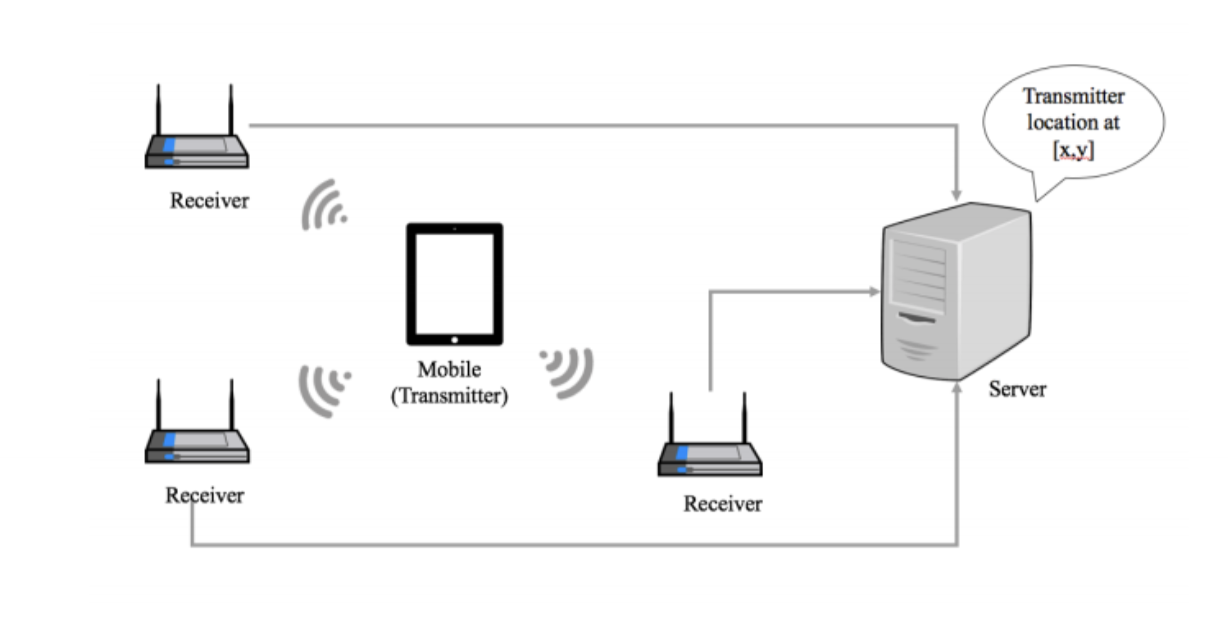
\includegraphics[width=\textwidth]{Image/remotepositioning.png}
\caption{Remote Positioning}
\label{fig:remote}
\end{figure}

\newpage
\subsection{Self Positioning}
\paragraph{}The mobile device will receive the signal from all transmitters. However, the location of all transmitters must be fixed and the mobile device must know where is the all transmitted located. After receiving the signal, the mobile device will act like the center station to calculates its positioning according to the location of transmitters. The overview of self positioning system is show in Figure~\ref{fig:self_positioning}

\begin{figure}[h]
\centering
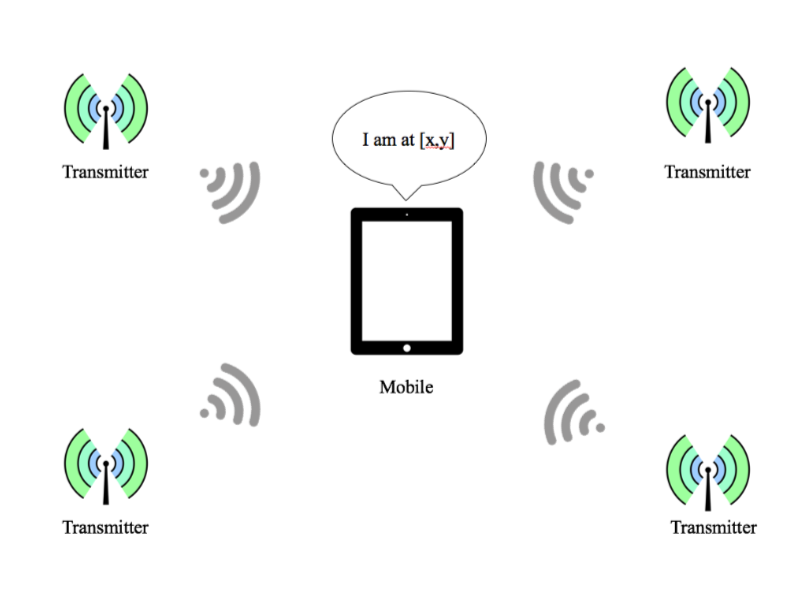
\includegraphics[scale = 0.6]{Image/selfpositioning.png}
\caption{Self Positioning}
\label{fig:self_positioning}
\end{figure}

\newpage
\subsection{Indirect Remote Positioning}
\paragraph{}The mobile device will receive the signal from several transmitters with know the exactly location as same as the self positioning topology. After that the mobile device will calculate the location of itself and send to the remote location. The overview of indirect remote positioning system show in Figure~\ref{fig:indirect_remote}

\begin{figure}[h]
\centering
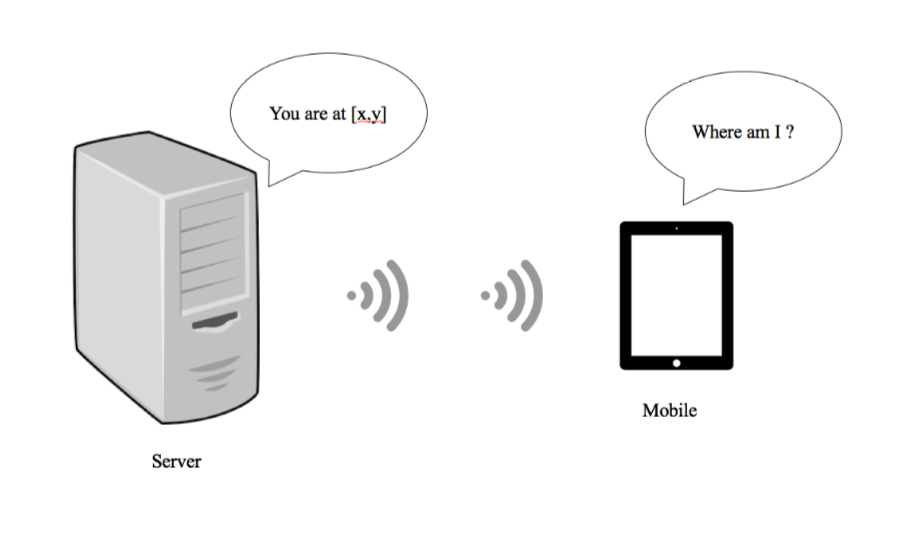
\includegraphics[width=\textwidth]{Image/indirect.png}
\caption{Indirect Remote Positioning}
\label{fig:indirect_remote}
\end{figure}


\newpage
\subsection{Indirect Self Positioning}
\paragraph{} The server collected signal with fixed measuring units from the mobile device. Then the measurement result from the measuring unit will be sent to the mobile device. In short, it is a remote positioning system that transmitting mobile device’s location to the mobile device. Figure~\ref{fig:indirect_self} depicts the overview of indirect self positioning system.

\begin{figure}[h]
\centering
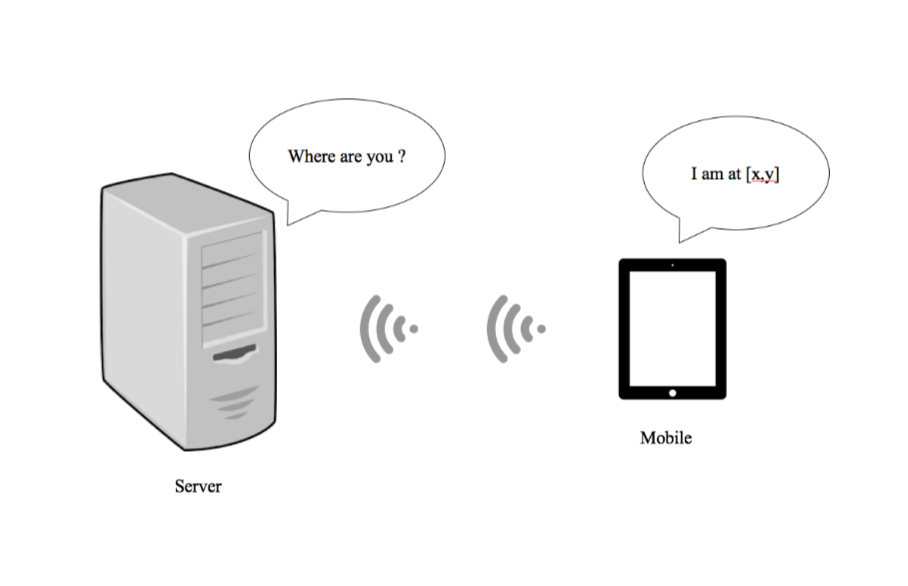
\includegraphics[width=\textwidth]{Image/direct.png}
\caption{Indirect Self Positioning}
\label{fig:indirect_self}
\end{figure}

\newpage
\section{Topology of Outdoor positioning}
\paragraph{}
The Outdoor Positioning Systems could be classified into two categories which
are Global Positioning System (GPS), and cellular network
\subsection{Global Positioning System (GPS)}
\paragraph{}
 GPS is a satellite-based radio-navigation system. It is a global navigation satellite system that provides geolocation and time information to a GPS receiver anywhere on or near the Earth where there is an unobstructed line of sight to four or more GPS satellites. Obstacles such as mountains and buildings block the relatively weak GPS signals. The GPS does not require the user to transmit any data, and it operates independently of any telephonic or internet reception, though these technologies can enhance the usefulness of the GPS positioning information. The GPS provides critical positioning capabilities to military, civil, and commercial users around the world. The United States government created the system, maintains it, and makes it freely accessible to anyone with a GPS receiver.

\subsection{Cellular network}
\paragraph{}
Mobile communication systems such as GSM (Global Standard for Mobile Communications) or UMTS (Universal
Mobile Telecommunication System) are based on a set of cellular networks. Since some years location-based services
(LBS) are delivered by these cellular approaches. LBSs are made possible through a suitable relationship between the
cellular service provider, cellular networks and mobile user’s terminals, which work in synch, to locate the user (mobile
terminal), and then transfer the position data either upon the request or as a continuous stream. The major issue is to
locate the user with a required accuracy and limited latency

\newpage
\section{Positioning Methods}
\paragraph{}
There are many methods have been researched for indoor and outdoor positioning. In this section, it can divided method into three positioning methods;  triangulation, trilateration, and fingerprint-based method. In additional, those locate objects by measuring signals. The main type of signal used in indoor positioning are infrared(IR) and radio frequency(RF) signal and this thesis will focus on using Bluetooth signal which is one type of RF signal.

\subsection{Triangulation}
\paragraph{}Triangulation estimation is a trigonometric approach of determining an unknown location based on two angles and a distance between them. Two or more fixed nodes are required for location estimate by receiving mobile signal (Bluetooth signals) from the signal-transmitting device. Furthermore, angle of Arrival(AoA) is a technique used in triangulation, this technique determines the angle of arrival of the mobile signal sent from the signal-transmitting device at which it is received by multiple receivers. From Figure~\ref{fig:aoa}, the location of the target node T1 is determined by measuring the angles of incidence (q1, q2) at which signals are sent from T1 and arrive at the receiving nodes R1 and R2. Geometric relationships can be used to calculate the coordinate (X,Y) of the target node.
\begin{figure}[h]
\centering
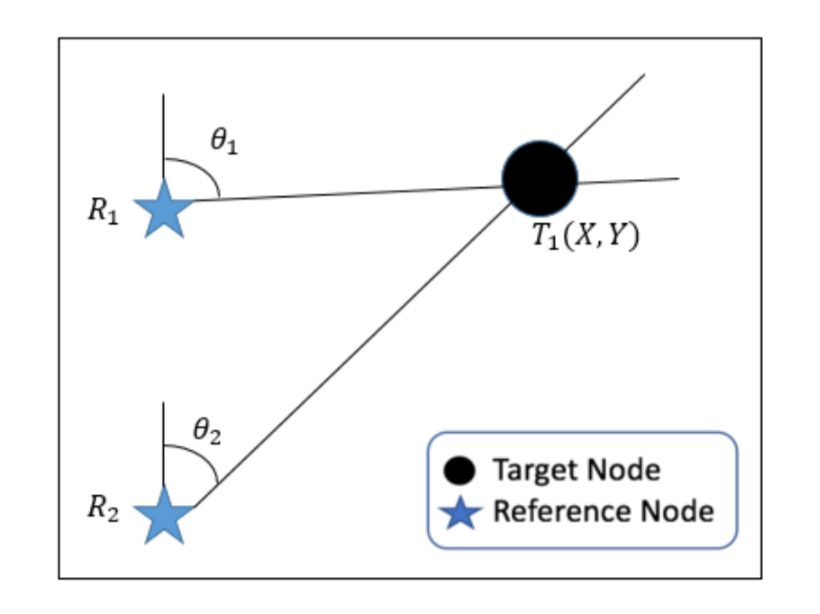
\includegraphics[scale = 0.7]{Image/triangulation.png}
\caption{Angle of Arrival}
\label{fig:aoa}
\end{figure}

\subsection{Trilateration Method}
\paragraph{}Trilateration is a traditional method to compute the unknown position of a node. At least three reference nodes with known positions are required in this method. Besides, the distances between these nodes and the mobile node are required to be known as well. Theoretically, each reference node forms a circle around itself with the radius of the distance to the mobile node. The position of the unknown node corresponds with the intersection of these three circles. Figure~\ref{fig:tri}, where the coordinate of the target object (X,Y) can be estimated using the coordinates of the receivers ((X1,Y1), (X2,Y2) and (X3,Y3)) and the distances (d1, d2 and d3).  Trilateration can be subdivided into two categories namely time-based method and RSSI-based method
\begin{figure}[h]
\centering
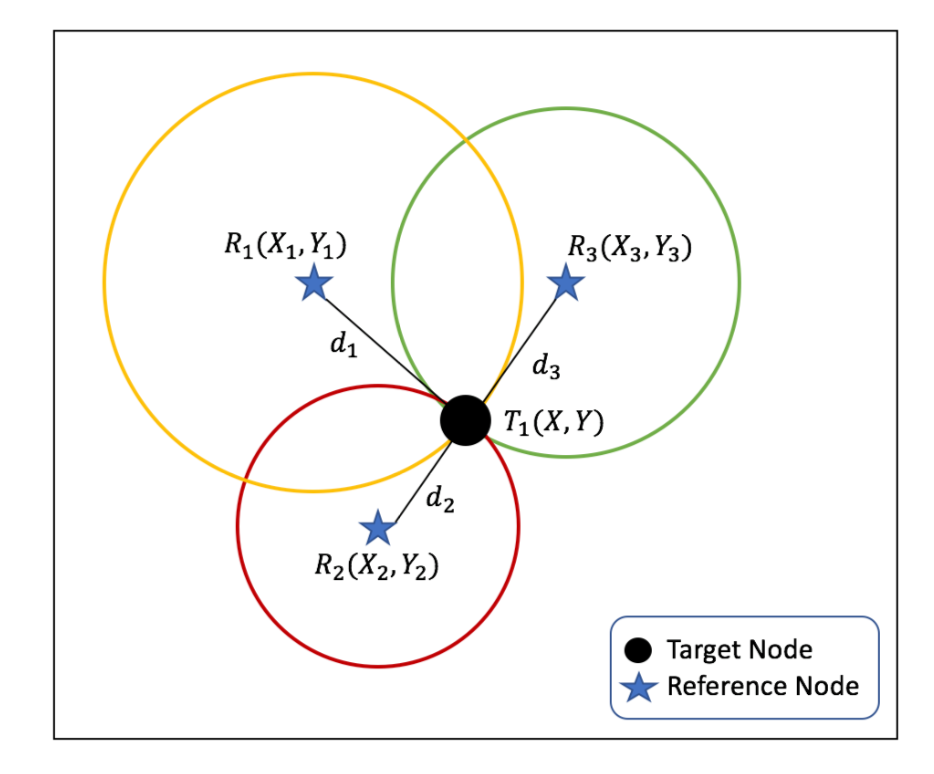
\includegraphics[scale = 0.7]{Image/trileteration.png}
\caption{Trilateration}
\label{fig:tri}
\end{figure}

\newpage
\subsection{Fingerprint-Based Method}
\paragraph{}Fingerprint-Based method is one of the popular techniques for indoor positioning due its high accuracy. The process of the fingerprint method consist of two main phases: training phase and classification phase. During the training phase we have to collect the RSSI data from each room of the target location and map the data into a classification model. After that, we train our system with the model we previously created. Next we go to the classification phase. In this phase the system will receive an input, which will be a RSSI sent from the target object, then it will classify the location of the target object via the model that it had learned. The fingerprint method can be a very accurate method with the use of a massive amount of data in the training phase. With that come a major disadvantage: it requires a lot of set up during the training phase. We need to collect large amount of data in order to just tell what room the device is in. To be able to track the device location with more precision the setup will be too impractical to be beneficial. And also the model that we use to train the system have to be proprietary to each location.


